%%%%%%%%%%%%%%%%%%%%%%%
%%% DOCUMENT SETTINGS
%%%%%%%%%%%%%%%%%%%%%%%
\documentclass[11pt]{exam}
%\printanswers % Uncomment to show answers
%%%%%%%%%%%%%%
%%% PACKAGES
%%%%%%%%%%%%%%
\usepackage{amsmath,amsfonts,amssymb,amsthm} % math fonts and symbols
\usepackage{bbm} % Math blackboard font
\usepackage{enumitem} % For reference enumerations lists
\usepackage{textcomp} % some symbols (like copyright)
\usepackage[top = 2cm, bottom = 2cm, right = 1.2cm, left = 1.2cm, paper = a4paper, headheight = 6cm]{geometry} % Margins setup
\usepackage{xcolor} % Colors
\usepackage{graphicx}
%----------------------------------- Tikz
\usepackage{tikz}
\usepackage{pgfplots}
\pgfplotsset{compat=1.17}
\usepgfplotslibrary{fillbetween}
\usetikzlibrary{shapes,arrows,matrix,positioning,calc}
\newcommand{\tikzmark}[1]{\tikz[baseline,remember picture] \coordinate (#1) {};}
%%%%%%%%%%%%%%%%%%%%%%%%%%
%%% Colors
%%%%%%%%%%%%%%%%%%%%%%%%%%
\definecolor{firebrick3}{RGB}{207, 33, 32}
\definecolor{deepskyblue3}{RGB}{0, 155, 206}
\definecolor{darkolivegreen3}{RGB}{163, 207, 91}
%%%%%%%%%%%%%%%%%%%%%%%%%%
%%% MACROS AND COMMANDS
%%%%%%%%%%%%%%%%%%%%%%%%%%
\newcommand{\N}{\mathbb{N}} % natural number set
\newcommand{\R}{\mathbb{R}} % real number set
\makeatletter
\renewcommand{\@makefnmark}{\textsuperscript{\arabic{footnote}}} % Ensure numeric superscripts
\renewcommand{\thefootnote}{\arabic{footnote}} % Ensure numeric labels
\makeatother
\setcounter{footnote}{0}
\newcommand{\BAR}{%
    \hspace{-\arraycolsep}%
    \strut\vrule % the `\vrule` is as high and deep as a strut
    \hspace{-\arraycolsep}%
}
%%%%%%%%%%%%%%%%%%%%%%%%%%%%%%%%%
%%% HEADER AND FOOT 
%%%%%%%%%%%%%%%%%%%%%%%%%%%%%%%%%
% Defining information
\newcommand{\degree}{Bachelor in Philosophy, Politics and Economics}
\newcommand{\shortdeg}{PPE}
\newcommand{\exam}{Final Exam}
\newcommand{\subject}{Mathematics}
\newcommand{\theyear}{2024/25}
\newcommand{\ccauthor}{A. G. Azze}
\newcommand{\thedate}{Dec 9, 2024}
\newcommand{\university}{CUNEF Universidad}
% Setting header and footer
\pagestyle{headandfoot}
\header{\degree \\ \subject\ - \theyear}{}{\thedate \\ \ccauthor}
\footer{\university}{}{\thepage}
%%%%%%%%%%%%%%%%%%%%%%%%%
%%% DOCUMENT CONTENT
%%%%%%%%%%%%%%%%%%%%%%%%%
\begin{document}
%--- Instructions ---%
\begin{center}

    {\Huge \textbf{\exam{}}}
   

    \begin{flushright}
        \vspace{-0.3cm}
        \textbf{Time Limit:} 120 minutes
    \end{flushright}
    \vspace{-0.3cm}
    
    \fbox{\parbox{\textwidth}{\centering 
        \begin{enumerate}[leftmargin = 0.5cm, label = $\bullet$, rightmargin = 0.2cm]
    
            \item \textbf{Every non-trivial calculation and claim in the exam must be properly justified.}

            \item The use of calculators is not necessary and therefore not allowed.

            \item Digital devices such as mobile phones, tablets, and laptops, as well as internet access, are forbidden.
            
        \end{enumerate}
    }}
\end{center}
%--- Instructions ---%

%--- Questions ---%

\begin{questions}

% Question
\question[3]
The whiskey market is described by the supply and demand functions $p_S(q) = (q^2 + 2q + 27)/5$ and $p_D(q) = 15 - q^2 - 2q$, respectively.

\begin{minipage}{0.51\textwidth}
    \begin{enumerate}[leftmargin = 0.5cm, label = (\alph*), rightmargin = 0.2cm]
        \item Check that there is a supply-demand equilibrium \\ at $(q^*, p^*) = (2, 7)$.
        \item Compute the consumer surplus (Area $C$ in Figure 1).
        \item Compute the area denoted by $A$ in Figure 1.
    \end{enumerate}
\end{minipage}
\hspace{0.8cm}
\begin{minipage}{0.35\textwidth}
    \vspace{-0.5cm}
    
    \begin{center}
    
    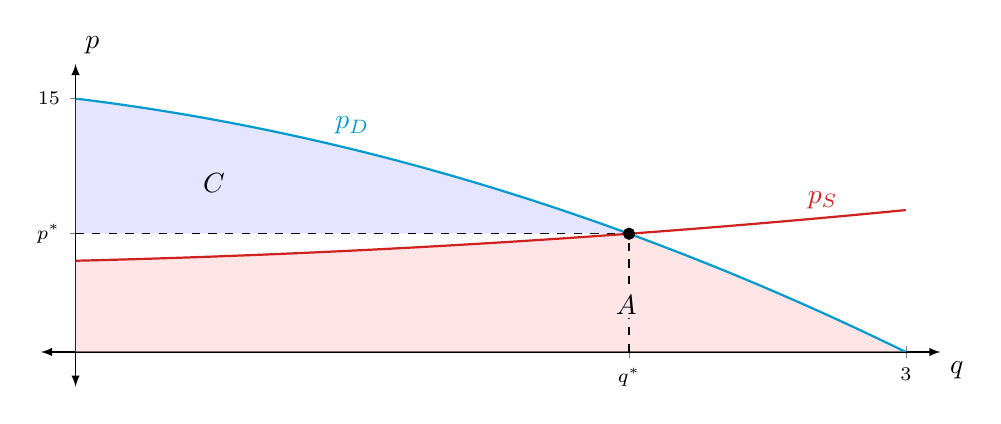
\begin{tikzpicture}

    % Axis
    \begin{axis}[
        width=\textwidth,
        height=4.8cm,
        axis lines=middle,
        xmin=0,
        xmax=3,
        ymin=0,
        ymax=15,
        ytick={0, 7, 15},
        xtick={0, 2, 3},
        xticklabels={$0$, $q^*$, $3$}, % Custom x-tick labels
        yticklabels={$0$, $p^*$, $15$}, % Custom y-tick labels
        scaled ticks = false,
        ticklabel style={font=\scriptsize},
        xlabel=$q$,
        ylabel=$p$,
        axis line style={
            latex-latex,
            shorten >=-12.5pt,
            shorten <=-12.5pt,
        },
        xlabel style={at={(ticklabel* cs:1)}, xshift=12.5pt, anchor=north west},
        ylabel style={at={(ticklabel* cs:1)}, yshift=12.5pt, anchor=south west},
    ]

    % Define the demand curve
    \path[name path=demand] plot[smooth, domain=0:2] (\x, {15 - \x^2 - 2*\x});
     % Define the price line
    \path[name path=price] (axis cs:0, 7) -- (axis cs:2, 7);
    % Consumer surplus area
    \addplot[fill=blue!20, opacity=0.5] fill between[
        of=demand and price,
    ];
    % Define the supply curve path from 0 to 2
    \path[name path=supply] plot[smooth, domain=0:2] (\x, {(27 + 2*\x + \x^2)/5});
    % Producer surplus area
    % \addplot[fill=green!20, opacity=0.5] fill between[
    %     of=supply and price,
    % ]; 
    % Define the x-axis (baseline) for supply
    \path[name path=xaxis_supply] (axis cs:0, 0) -- (axis cs:2, 0);
    % Define the demand curve path from 2 to 3
    \path[name path=demand_2_to_3] plot[smooth, domain=2:3] (\x, {15 - \x^2 - 2*\x});
    % Define the x-axis (baseline) for demand from 2 to 3
    \path[name path=xaxis_demand] (axis cs:2, 0) -- (axis cs:3, 0);
    % Fill the area under the supply curve from 0 to 2
    \addplot[fill=red!20, opacity=0.5] fill between[
        of=supply and xaxis_supply,
    ];
    % Fill the area under the demand curve from 2 to 3
    \addplot[fill=red!20, opacity=0.5] fill between[
        of=demand_2_to_3 and xaxis_demand,
    ];
    % Demand and Supply functions
    \addplot[thick, firebrick3, samples=51, smooth, domain=0:3] {(27 + 2*x + x^2)/5};
    \addplot[thick, deepskyblue3, samples=51, smooth, domain=0:3] {15 - x^2 - 2*x};
    % Equilibrium point
    \addplot[mark=*] coordinates {(2, 7)} node[] {};
    % Dashed lines to the equilibrium point
    \addplot[dashed] coordinates {(2, 4) (2, 7)}; % Vertical line
    \addplot[dashed] coordinates {(2, 0) (2, 2)}; % Vertical line
    \addplot[dashed] coordinates {(0, 7) (2, 7)}; % Horizontal line
    % Functions labels
    \addplot[] coordinates {(2.7, 9)} node[] {$\textcolor{firebrick3}{p_S}$}; 
    \addplot[] coordinates {(1, 13.4)} node[] {$\textcolor{deepskyblue3}{p_D}$};
    % Areas labels
    \addplot[] coordinates {(0.5, 10)} node[] {$C$}; 
    % \addplot[] coordinates {(0.165, 6.2)} node[] {$P$};
    \addplot[] coordinates {(1.99, 2.8)} node[] {$A$};
    
    \end{axis}
        
    \end{tikzpicture}
    \vspace{-0.6cm}
    
    {\small Figure 1}
    \end{center}        
\end{minipage}
\vspace{0.1cm}

The government applies a tax of $T$ dollars per unit of whiskey produced to lower its consumption and raise money, making the new equilibrium quantity $q^*(T) = \sqrt{\frac{54 - 3T}{3}} - 1$.
\begin{enumerate}[leftmargin = 0.5cm, label = (\alph*), rightmargin = 0.2cm]
    \item[(e)] What is the domain of $q^*(T)$? 
    \item[(f)] What is the continuity domain of $q^*(T)$?
    \item[(g)] For what value of $T$ the suppliers will not produce any unit of whiskey.
\end{enumerate}

\begin{minipage}{0.51\textwidth}
Denote by $R(T)$ to the government's profit after applying the whiskey tax policy. 
\begin{enumerate}[leftmargin = 0.5cm, label = (\alph*), rightmargin = 0.2cm]
    \item[(h)] Write a formula for $R(T)$ in terms of $q^*(T)$.
    \item[(i)] You are in charge of the tax policy and Figure 2 is handed to you. Which tax value would you impose?
    \item[(j)] Give an approximation of $R(0.1)$ provided that $R'(0) = 3\sqrt{2} -1$
\end{enumerate}
\end{minipage}
\hspace{0.8cm}
\begin{minipage}{0.38\textwidth}
    \vspace{-0.2cm}
    \begin{center}
    
    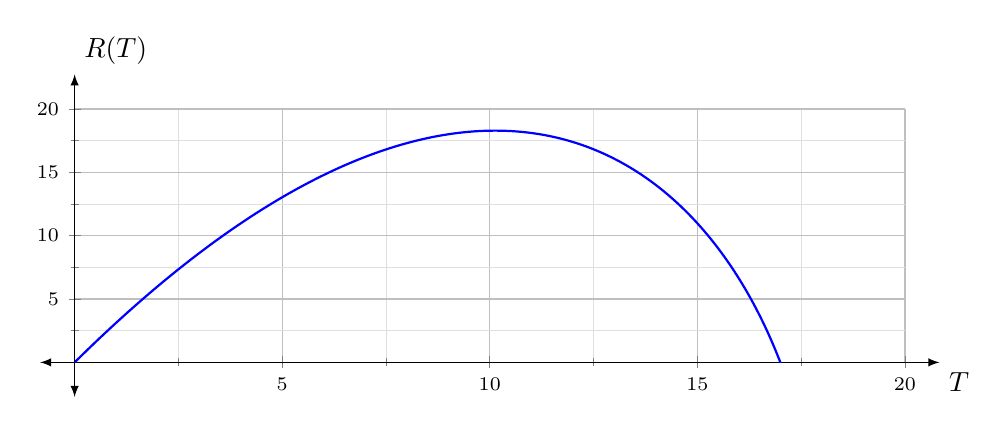
\begin{tikzpicture}

    % Axis
    \begin{axis}[
        width=\textwidth,
        height=4.8cm,
        axis lines=middle,
        xmin=0,
        xmax=20,
        ymin=0,
        ymax=20,
        xtick={0, 5, 10, 15, 20}, % Add tick marks from 0 to 18 on x-axis
        ytick={0, 5, 10, 15, 20}, % Add tick marks from 0 to 18 on y-axis
        grid=both,             % Add a mesh/grid
        minor tick num=1,      % Minor grid for better precision
        major grid style={line width=0.5pt, draw=gray!50},
        minor grid style={line width=0.25pt, draw=gray!25},
        ticklabel style={font=\scriptsize},
        xlabel=$T$,
        ylabel=$R(T)$,
        axis line style={
            latex-latex,
            shorten >=-12.5pt,
            shorten <=-12.5pt,
        },
        xlabel style={at={(ticklabel* cs:1)}, xshift=12.5pt, anchor=north west},
        ylabel style={at={(ticklabel* cs:1)}, yshift=12.5pt, anchor=south west},
    ]
    % Profit curve
   \addplot[
        domain=0:18,
        samples=500,
        blue,
        thick
    ] {x*(sqrt((54 - 3*x)/3) - 1)} node[pos=0.8, above] {};
    
    \end{axis}
        
\end{tikzpicture}
    \vspace{-0.5cm}
    
    {\small Figure 2: Government's tax profit}
    \end{center}
\end{minipage}
    
% Solution
\begin{solution}[0cm]
    \begin{enumerate}[leftmargin = 0.5cm, label = (\alph*), rightmargin = 0.2cm]
        
        \item Straightforward algebra leads to 
        $$
        p_S(2) = \frac{2^2 + 2\cdot2 + 27}{5} = \frac{35}{5} = 7, \quad p_D(2) = 15 - 2^2 - 2\cdot2 = 15 - 4 - 4 = 7.
        $$

        \item The consumer surplus takes the form
        \begin{align*}
            C &= \int_0^2 p_D(q) \, \mathrm{d}q - p^* q^* = \int_0^2 (15 - q^2 - 2q) \, dq - p^* q^* \\
            &= \left( 15q - \frac{q^3}{3} - q^2 \right)\Bigg|_0^2 - p^* q^* = 15\cdot2 - \frac{2^3}{3} - 2^2 - 2 \cdot 7 \\
            &= 30 - 4- 14- \frac{8}{3} = 12 - \frac{8}{3} = \frac{36 - 8}{3} = \frac{28}{3}.
        \end{align*}

        \item Note that the area $A$ is the sum of the area under $p_D(q)$ from $q = 0$ to $q = 2$ (call it $A_1$) and the area under $p_S(q)$ from $q = 2$ to $q = 3$ (call it $A_2$). We have that
        \begin{align*}
            A_1 &= \int_0^2 p_S(q) \, dq = \int_0^2 \frac{q^2 + 2q + 27}{5} \, dq 
            = \frac{1}{5} \left( \frac{q^3}{3} + q^2 + 27q \right)\Bigg|_0^2 \\
            &= \frac{1}{5} \left( \frac{2^3}{3} + 2^2 + 27\cdot2 \right) 
            = \frac{1}{5} \left( \frac{8}{3} + 58 \right) = \frac{1}{5} \frac{182}{3} = \frac{182}{15},
        \end{align*}
        and
        \begin{align*}
            A_2 &= \int_2^3 p_D(q) \, dq = \int_2^3 (15 - q^2 - 2q) \, dq 
            = \left( 15q - \frac{q^3}{3} - q^2 \right)\Bigg|_2^3 \\
            &= \left( 15\cdot3 - \frac{3^3}{3} - 3^2 \right) - \left( 15\cdot2 - \frac{2^3}{3} - 2^2 \right) \\
            &= \left( 45 - 9 - 9 \right) - \left( 30 - \frac{8}{3} - 4 \right) = 27 - \frac{70}{3} = \frac{81 - 70}{3} = \frac{11}{3}.
        \end{align*}
        Hence, 
        $$
        A = \frac{182}{15} + \frac{11}{3} = \frac{182+55}{3} = \frac{237}{15} = \frac{79}{5}.
        $$

        \item The domain of $q^*(T)$ are all the values of $T$ that makes the expression within the square root non-negative, that is $(-\infty, 18]$, although we main consider the effective domain as $[0, 18]$, since $T$ must be positive as it represents a tax quantity.

        \item The function $q^*(T)$ is continuous in all its domain.

        \item Note that
        \begin{align*} 
            \sqrt{\frac{54 - 3T}{3}} - 1 = 0 \Longleftrightarrow \frac{54 - 3T}{3}  = 1 \Longleftrightarrow T = 17.
        \end{align*}

        \item $R(T) = Tq^*(T)$.

        \item $T^*\approx 10$ is an optimal choice, since the function $R(T^*)$ reaches its global maximum at that point.

        \item We know that $R(0 + 0.1) \approx R(0) + R'(0)(0.1 - 0) = (3\sqrt{2} -1)0.1 \approx 0.3243$. To appreciate the accuracy of the approximation, $R(0.1) \approx 0.3231$.
        
    \end{enumerate}
\end{solution}


% Question
\question[2]

As a bar owner, you plan to stock $x$ $4$-servings bottles of whiskey, $y$ $6$-servings bottles of wine, and $z$ $8$-servings bottles of rum, for a total of $20$ bottles. When fully stocked, you want to the bottles to hold a total of $108$ servings. In the quite season you want to be able to provide a total of $46$ servings with a stock of only half of the whiskey bottles, half of the wine bottles, and one-fourth of the rum bottles. 

\begin{enumerate}[leftmargin = 0.5cm, label = (\alph*), rightmargin = 0.2cm]
    \item Write the system of equations necessary to find $x$, $y$, and $z$.
    \item Express the system in matrix form, that is, find a matrix $A$ and a vector $\pmb{b}$ such that $A\pmb{w} = \pmb{b}$, for $\pmb{w} = (x, y, z)$ 
    \item Assume that 
    $A^{-1} =
    \begin{pmatrix}
        3 & -0.25 & -0.5 \\
        -2 & 0 & 1 \\
        0 & 0.25 & -0.5
    \end{pmatrix}$. 
    Find the value of $x$, $y$, and $z$. 
    \item What would be the answer if you knew that the determinant of $A$ is zero?
\end{enumerate}

% Solution
\begin{solution}[0cm]
    \begin{enumerate}[leftmargin = 0.5cm, label = (\alph*), rightmargin = 0.2cm]
        
        \item The system of linear equations is
        \begin{align*}
            x + y + z &= 20  && \text{(Total number of bottles)} \\
            4x + 6y + 8z &= 108 && \text{(Total number of servings)} \\
            2x + 3y + 2z &= 46 && \text{(Servings during the quiet season)}
        \end{align*}

        \item The matrix $A$ and vector $\pmb{b}$ are
        \begin{align*}
            A = 
            \begin{pmatrix}
                1 & 1 & 1 \\
                4 &  6 &  8 \\
                2 &  3 & 2
            \end{pmatrix}, \quad
            \pmb{b} = 
            \begin{pmatrix}
                20 \\
                108 \\
                46
            \end{pmatrix}
        \end{align*}

        \item The solution can be obtained by performing the matrix multiplication $A^{-1}\pmb{b}$, which yields $x = 10$, $y = 6$, $z = 4$.

        \item In such a case $A$ would have no inverse and the system would have either no solution or infinitely many solutions.
        
    \end{enumerate}
\end{solution}

% Question
\question[3]
     You own a barrel of whiskey whose initial price in the market is $K = 100$ dollars. As the whiskey gets older, its price increases, such that the barrel price after $t$ years is given by $W(t) = K\sqrt{t}$. On the other hand, the inflation rate of the country makes future profits decrease at a rate such that $x$ dollars today equals $x/(1 + t)$ dollars $t$ years from now. 

    \begin{enumerate}[leftmargin = 0.5cm, label = (\alph*), rightmargin = 0.2cm]
        
        \item Obtain the function $P(t)$ that determines the whiskey barrel price after $t$ years.

        \item What would be the discounted value of the whiskey barrel after an infinite amount of time?

        \item When should you sell the whiskey to maximize your profit and what would be that optimal profit? \\
        You may find useful the fact that $P'(t) = 50\frac{t^{-1/2}(1 - t)}{(1 + t)^2}$.

        \item If you are forced to sell the barrel before a time horizon $T$, would your optimal time to sell would change if $T = 0.5$? Would it change for $T = 2$? Why?
        
    \end{enumerate}
    
%% Solution
\begin{solution}[0cm]
    \begin{enumerate}[leftmargin = 0.5cm, label = (\alph*), rightmargin = 0.2cm]
        \item $P(t) = \frac{W(t)}{(1+t)} = K \frac{\sqrt{t}}{1+t}$.
        \item The value would be $\lim_{t\rightarrow\infty} P(t) = 0$.
        \item Note that $P'(t) = 0 \Longleftrightarrow t = 1$. Also, $P'(t) > 0$ for all $t\in(0, 1)$ and $P'(t) < 0$ for all $t\in(1, \infty)$ meaning that $P$ reaches a global maximum at $t = 1$ and, therefore, it is optimal to sell at that time, making a profit of $P(1) = 50$ dollars.
        \item The same reasoning we used in the previous part yields that the global maximum of $P(t)$ constrained to $t\in[0, 0.5]$ is reached at $0.5$, meaning that in such a case the optimal time to sell does change compared to the unconstrained problem. For the case $T = 2$ the optimal time remains the same as in the unconstrained problem, since $t = 1$ is still a valid time within the interval $[0, 2)$.         
    \end{enumerate}
\end{solution}

% Question
\question[2]
The ``Whiskey, Inc.'' company issues perpetual bonds\footnote{Also called consol, this is a type of bond that pays fixed or variable dividends forever} with different continuous dividend-paying schemes. For all cases, the present value of the bond associated by the dividend profile $D(t)$ is given by $V = \int_{0}^{\infty} D(t) e^{-rt} \, \mathrm{d} t$, where $r > 0$ is the discount rate. Take $r = 1$ and answer the following questions:
\begin{enumerate}[leftmargin = 0.5cm, label = (\alph*), rightmargin = 0.2cm]
   \item \textbf{Constant Dividend:} $D(t) = 1$. What is the value of $V$?
   \item \textbf{Exponentially Growing Dividend:} $D(t) = e^{\alpha t}$, where $\alpha > 0$ is the growth rate of the dividend. Obtain the value of $V$ for
   \begin{enumerate}[leftmargin = 0.5cm, label = (\roman*), rightmargin = 0.2cm]
        \item $\alpha = 0.5$;
        \item $\alpha = 2$.
   \end{enumerate}
   \item \textbf{Linearly Increasing Dividend:} $D(t) = (1 + \beta t)$, where $\beta > 0$ is the linear growth coefficient. What\footnote{You may find useful the fact that the primitive (anti-derivative) of the function $(1 + \beta t)e^{-t}$ is $-\left( 1 + \beta + \beta t \right)e^{-t} + C$, for a constant $C$.} is the value of $V$? 
   \item \textbf{Oscillating Dividend:} $D(t) = |\cos(t)|$. Find\footnote{Hint: use the fact that $-1 \leq \cos(t) \leq 1$} a number $K$ such that $V < K$.
\end{enumerate}

%% Solution
\begin{solution}[0cm]

    \begin{enumerate}[leftmargin = 0.5cm, label = (\alph*), rightmargin = 0.2cm]
        \item Using the formula $V = \int_{0}^{\infty} D(t) e^{-rt} \, \mathrm{d} t$ for $D(t) = 1$,
        \begin{align*}
            V = \int_0^\infty e^{-t} \, dt = \lim_{b\rightarrow\infty} -e^{-t}\big|_0^b = \lim_{b\rightarrow\infty} (1-e^{-b}) = 1
        \end{align*}

        \item The general formula in this case is $V = \int_0^\infty e^{\alpha t} e^{-t} \, dt = \int_0^\infty e^{(\alpha - 1)t} \, dt$. Hence,
        \begin{align*}
            V &= \int_0^\infty e^{-t/2} \, dt = \lim_{b\rightarrow\infty} -2e^{-t/2}\big|_0^b = \lim_{b\rightarrow\infty} 2(1-e^{-b/2}) = 2 & (i), \\
            V &= \int_0^\infty e^{t} \, dt = \lim_{b\rightarrow\infty} e^{t}\big|_0^b = \lim_{b\rightarrow\infty} (1-e^{b}) = \infty. & (ii).\\
        \end{align*}

        \item From the hint, 
        \begin{align*}
            V &= \int_0^\infty \frac{e^{-t}}{1+t} \, dt 
            = \lim_{b\rightarrow\infty} -\left( 1 + \beta + \beta t\right)e^{-rt}\Bigg|_0^b
            = \lim_{b\rightarrow\infty} \left((1 + \beta) - \left( 1 + \beta + \beta b\right)e^{-rb}\right) = 1 + \beta.
        \end{align*}

        \item From the hint, $|\cos(t)| \leq 1$. Hence,
        \begin{align*}
            V &= \int_0^\infty |\cos(t)|e^{-t} \, dt \leq \int_0^\infty e^{-t} \, dt = 1.
        \end{align*}
    \end{enumerate}
\end{solution}

\end{questions}	

\end{document}